% !TeX spellcheck = en_GB
\documentclass[9pt,twocolumn,twoside,lineno]{pnas-new}
% Use the lineno option to display guide line numbers if required.

\templatetype{pnasresearcharticle}

\title{Public Perceptions on the Coal Debate on Twitter: Reactions to a Corporate Decision-Making Policy Process}

% Use letters for affiliations, numbers to show equal authorship (if applicable) and to indicate the corresponding author
\author[a,b,1]{Yuan Ting Lee}

\affil[a]{Hertie School, Friedrichstr. 180, Berlin 10117, Germany}
\affil[b]{Mercator Research Institute on Global Commons and Climate Change, Torgauer Str. 19, Berlin 10829, Germany}

% Please give the surname of the lead author for the running footer
\leadauthor{Lee} 

% Please include corresponding author, author contribution and author declaration information
\authorcontributions{}
\authordeclaration{}
\equalauthors{}
\correspondingauthor{\textsuperscript{1}To whom correspondence should be addressed. E-mail: y.lee@mpp.hertie-school.org}

% Keywords are not mandatory, but authors are strongly encouraged to provide them. If provided, please include two to five keywords, separated by the pipe symbol, e.g:
\keywords{Keyword 1 $|$ Keyword 2 $|$ Keyword 3 $|$ ...} 

\begin{abstract}
Please provide an abstract of no more than 250 words in a single paragraph. Abstracts should explain to the general reader the major contributions of the article. References in the abstract must be cited in full within the abstract itself and cited in the text.
\end{abstract}

\dates{This manuscript was compiled on \today}

\begin{document}

\maketitle
\thispagestyle{firststyle}
\ifthenelse{\boolean{shortarticle}}{\ifthenelse{\boolean{singlecolumn}}{\abscontentformatted}{\abscontent}}{}

\dropcap{M}ulti-stakeholder commissions have been an important instrument for incorporating external expertise into political decision-making in Germany. It can be seen as an element of “negotiation democracy”, whereby the experts in the commission decide on an outcome via deliberations and negotiations. Depending on the policy field, representatives of business, science, the social partners, churches, associations and societies can be appointed and thus accelerate the later public discussion. \cite{Siefken2016}

The Coal Commission, formally known as the Commission on Growth, Structural Change and Employment, is such an example of expert commissions. It was set up by the German government under the Federal Ministry for Economy and Energy (BMWi), and was tasked with developing an overarching approach to managing the coal phase-out’s technical, legal, economic and social impacts.

Criticisms have emerged about the process of the coal commission, namely that ....

The process of the German coal commission thus presents a unique situation for analysis: is there a relationship between the seemingly "corporatist" process of such an expert commission and public opinion, as represented on social media, on the topic? Here, tweets from Twitter are used to represent public opinion on social media, in part due to their high granularity which allows for observations on swiftly changing temporal patterns on topic salience.

\section*{Related Work}


\section*{Task}

\section*{Data}
The data used in this project was collected via a two-part process, using two python packages: \texttt{twint} to download the tweets based on specific queries, and \texttt{tweepy} to populate the tweets with extended tweet information. %be more specific and clear here

% insert figure on data collection

The selection process for choosing tweets to analyse stems from the research question at hand, which is to understand the greater coal debate in Germany on Twitter. The final collection of tweets thus include two sets of tweets collected using two different search strategies. The first search strategy includes terms that directly relate to the coal exit in Germany - \{Kohlekommission, Kohleausstieg, Kohlefrei\}.\footnote{Translation: Coal commission, Coal exit, Coal free}

The other set of tweets is obtained from a general search for tweets on coal ("Kohle"), which are then filtered by the inclusion of relevant hashtags in the text of the tweets. These relevant hashtags are obtained by conducting a frequency analysis of all hashtags that appear in "Kohle" tweets, and manually selecting the top hashtags that are related to coal in climate policy. These hashtags are:  \{\#Klimaschutz, \#Hambacherforst, \#Hambibleibt, \#endcoal, \#fridaysforfuture, \#klimawandel, \#klima, and \#endegelaende\}.\footnote{Translation: Climate policy, Hambach Forest, Stay Hambach (forest), Climate Change, Climate,} 

The two collections are then combined and duplicates are removed, and the final set is then filtered for tweets in German, which can be obtained as a result from querying the Twitter API. 

\begin{figure} 
	\begin{center}
		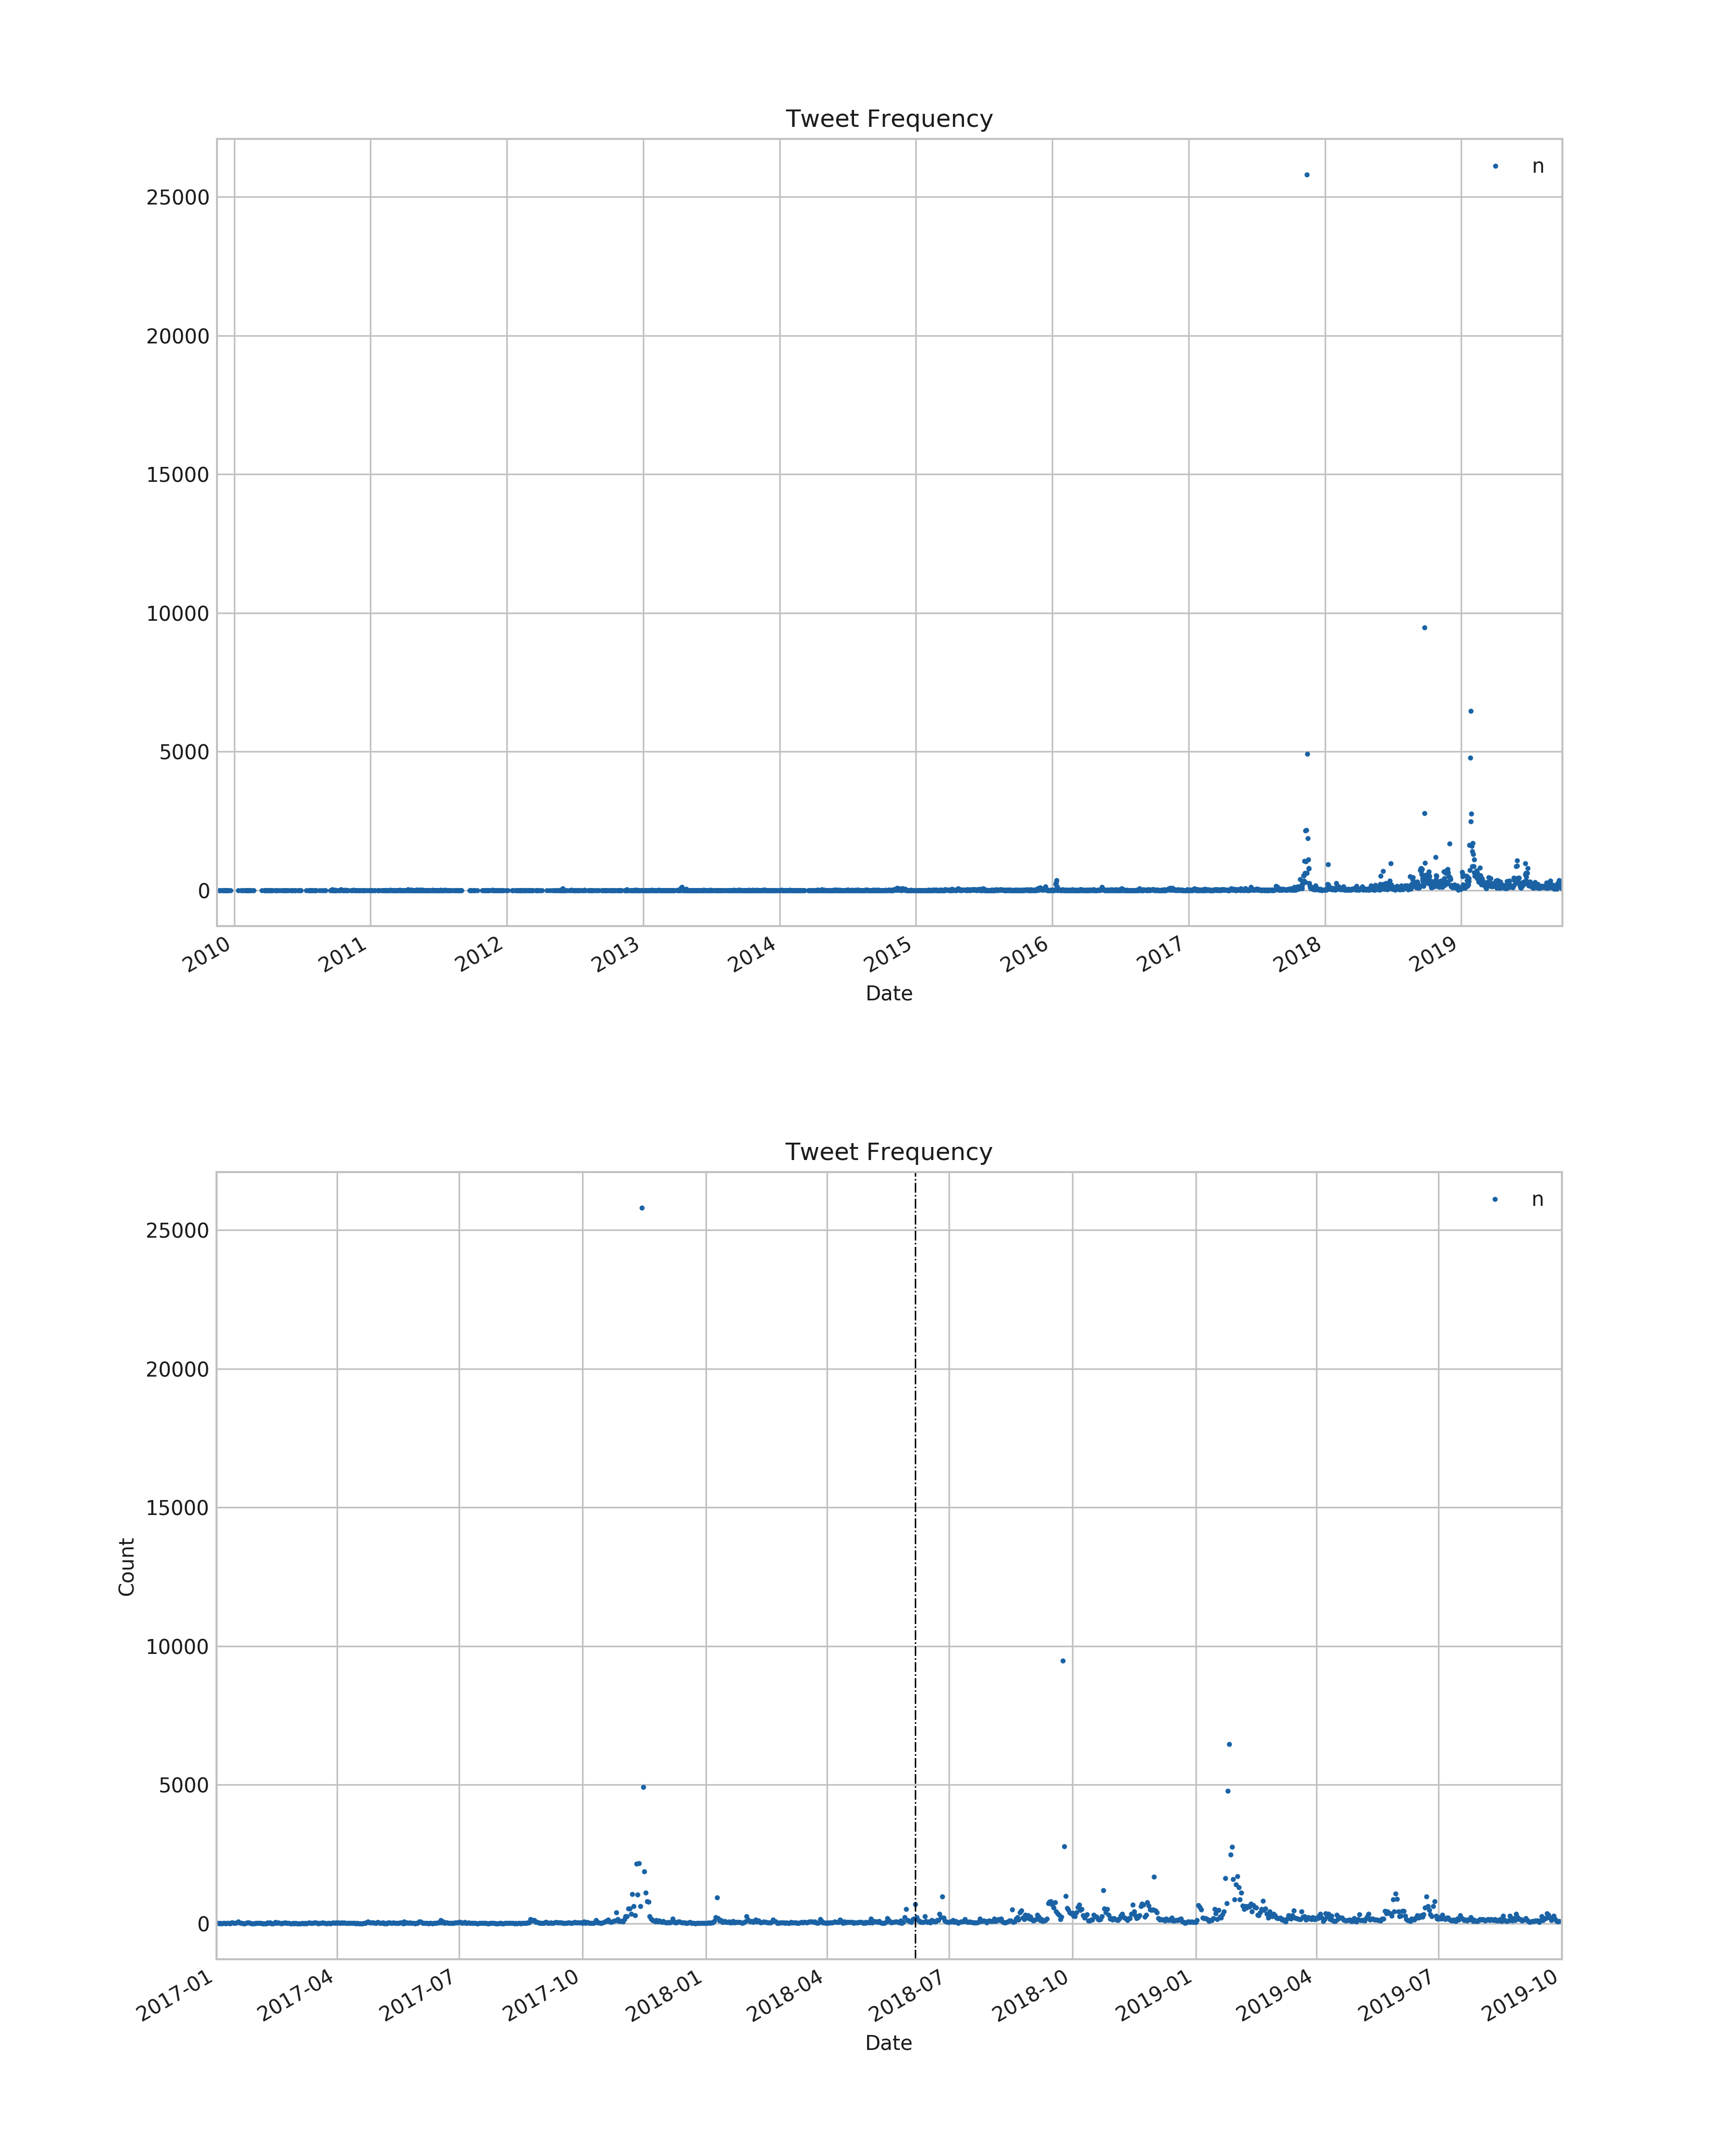
\includegraphics[width=\linewidth]{figures/tweet_frequency_combine}
	\end{center}
	\caption{Daily frequency of tweets in combined dataset}
	\label{fig:tweet_frequency}
\end{figure}


\section*{Proposed Method}
% Explanation of sentiment analysis 

Sentiment analysis refers to the use of natural language processing and text analysis to systematically identify and extract affective states and subjective information in text. % cite?

The dictionary used is SentiWS - \cite{REMUS10.490}

To obtain the sentiment score of a tweet, denoted by \(s_{tweet}\), the following formula is used: \[s_{tweet} = \frac{\sum_{i=1}^{n} s_i f_i}{\sum_{i=1}^{n} f_i}\] where \(s_i\) is the polarity weighting score of a word given in SentiWS, and \(f_i\) is the frequency of occurrence of the word in the tweet. 

\section*{Results}

\begin{figure} 
	\begin{center}
		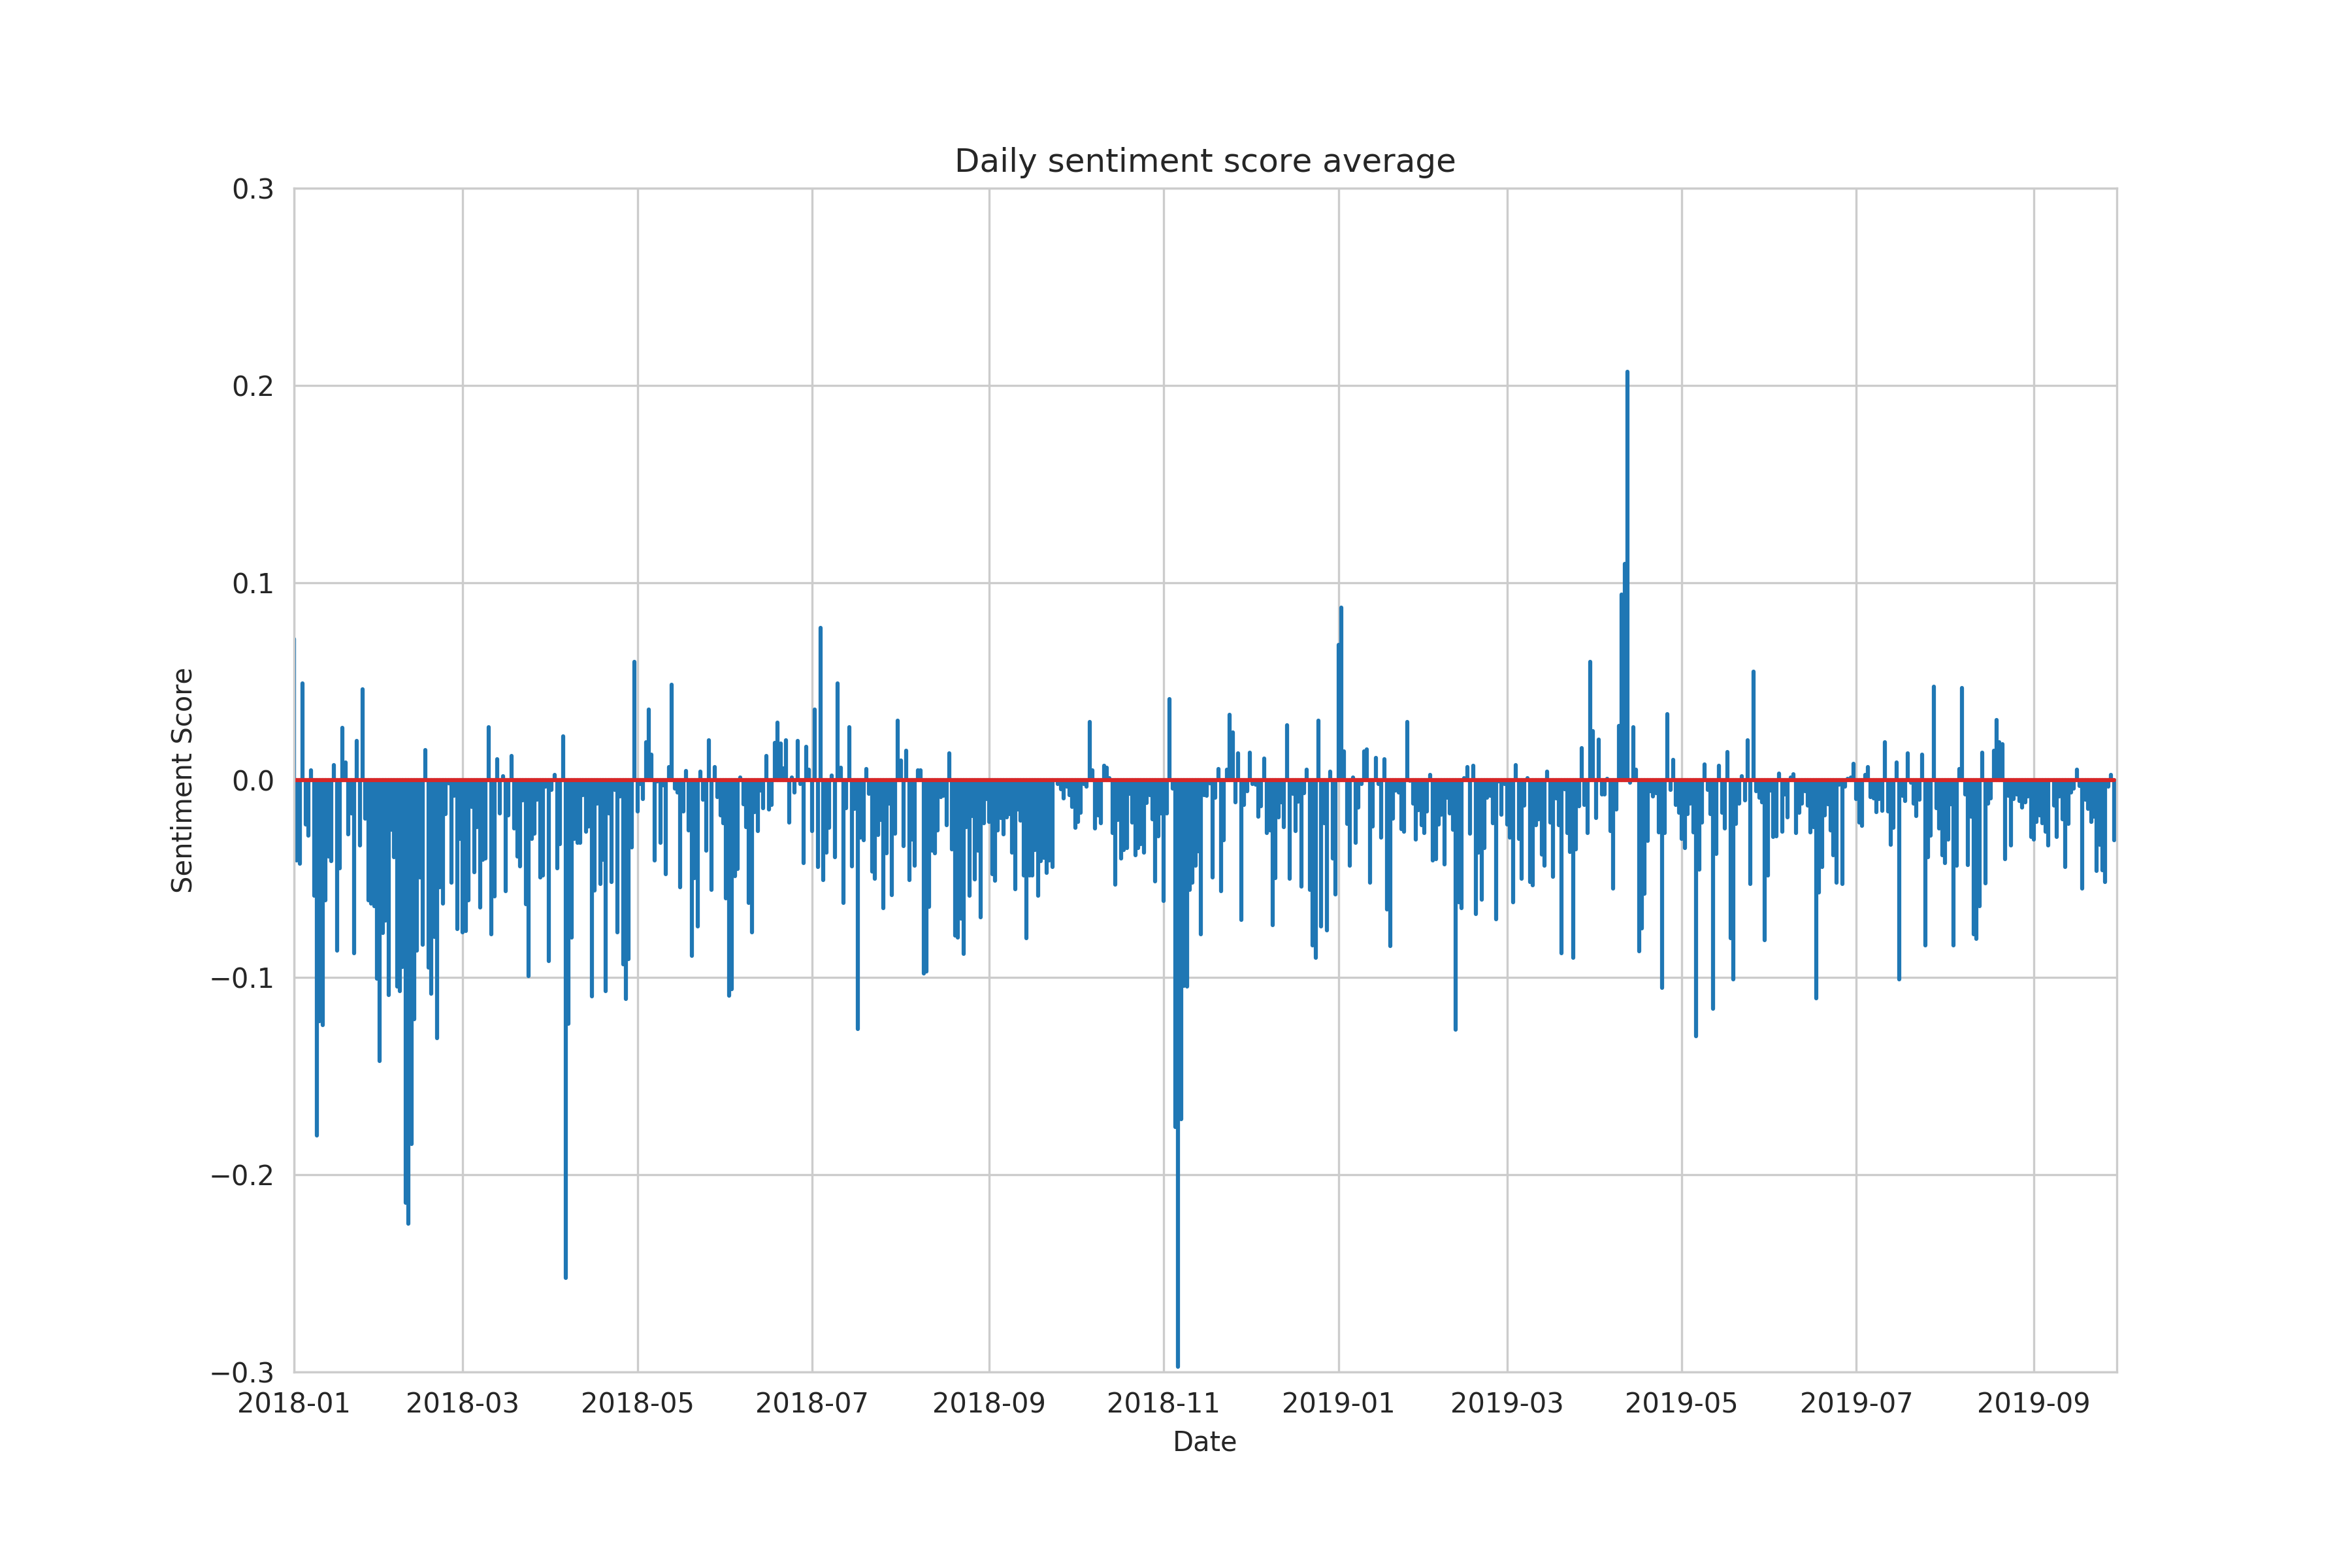
\includegraphics[width=\linewidth]{figures/dailyavgsenti}
	\end{center}
	\caption{Daily average sentiment score of tweets}
	\label{fig:tweet_score}
\end{figure}



\subsubsection*{SI Datasets} 


\subsubsection*{SI Movies}


\subsubsection*{3D Figures}


\matmethods{Please describe your materials and methods here. This can be more than one paragraph, and may contain subsections and equations as required. Authors should include a statement in the methods section describing how readers will be able to access the data in the paper.}

\subsection*{Subsection for Method}
Example text for subsection.


\showmatmethods{} % Display the Materials and Methods section

\acknow{Please include your acknowledgments here, set in a single paragraph. Please do not include any acknowledgments in the Supporting Information, or anywhere else in the manuscript.}

\showacknow{} % Display the acknowledgments section

\section*{References}
% Bibliography
\bibliography{bibliography.bib}

\end{document}